
\documentclass[11pt,a4paper,sans]{moderncv}        % possible options include font size ('10pt', '11pt' and '12pt'), paper size ('a4paper', 'letterpaper', 'a5paper', 'legalpaper', 'executivepaper' and 'landscape') and font family ('sans' and 'roman')

% moderncv themes
\moderncvstyle{classic}                            % style options are 'casual' (default), 'classic', 'oldstyle' and 'banking'
\moderncvcolor{blue}                               % color options 'blue' (default), 'orange', 'green', 'red', 'purple', 'grey' and 'black'
%\renewcommand{\familydefault}{\sfdefault}         % to set the default font; use '\sfdefault' for the default sans serif font, '\rmdefault' for the default roman one, or any tex font name
%\nopagenumbers{}                                  % uncomment to suppress automatic page numbering for CVs longer than one page

% adjust the page margins
\usepackage[scale=0.76]{geometry}
\setlength{\hintscolumnwidth}{2.05cm}                % if you want to change the width of the column with the dates
%\setlength{\makecvtitlenamewidth}{10cm}           % for the 'classic' style, if you want to force the width allocated to your name and avoid line breaks. be careful though, the length is normally calculated to avoid any overlap with your personal info; use this at your own typographical risks...

\usepackage[normalem]{ulem}
\usepackage{color}
\usepackage{bm}
\usepackage{amstext}
\newcommand{\coloredLink}[2]{\textcolor{blue}{\href{#1}{#2}}}
\usepackage{tikzpagenodes}


\newcommand\ttbb{\ensuremath{t\bar{t}b\bar{b}}}
\newcommand\ttbar{\ensuremath{t\bar{t}}}
\newcommand\tttt{\ensuremath{t\bar{t}t\bar{t}}}
\newcommand\ttH{\ensuremath{t\bar{t}H}}
\newcommand\bbbar{\ensuremath{b\bar{b}}}
\newcommand{\met}{\ensuremath{E_{{T}}^{{miss}}}}
\newcommand{\pt}{\ensuremath{p_{T}}}

\newif\ifAddReferences  %% References
\newif\ifAddStatement  %% Statement of research interest
\newif\ifAddInternalTalks  %% References
\AddReferencesfalse
\AddStatementfalse
\AddInternalTalksfalse



\name{Javier}{Montejo Berlingen} %many FIXME around the CV, find them
%%%%%%%%%%%%%%%%%%%%%%
% SINCE YOU ARE READING THIS, LET ME REMIND YOU ABOUT THE IDEA OF HAVING A VERTICAL LINE IN THE MIDDLE
% AND THE RESULTS AND POSITIONS ON BOTH SIDES TO GIVE CONTEXT OF THE TIMELINE
%                                                                  CHECK 'CV nuevo layout.key' <----------
%%%%%%%%%%%%%%%%%%%%%%
\title{CERN Staff Physicist}                               % optional, remove / comment the line if not wanted
%\address{CERN 40/5-C11}{1217 Meyrin}{Switzerland}
%\phone[fixed]{+41~786314562}
%\email{jmontejo@cern.ch}                               % optional, remove / comment the line if not wanted


\usepackage{multibib}
\newcites{article,confnote,proceedings}{{Articles},{Conference Notes},{Proceedings}}

%----------------------------------------------------------------------------------
%            content
%----------------------------------------------------------------------------------
\begin{document}
%-----       resume       ---------------------------------------------------------
\makecvtitle
\vspace*{-15mm}

\begin{tikzpicture}[remember picture,overlay,shift={(current page.north east)}]
\node[anchor=north east,xshift=-2cm,yshift=-2cm]{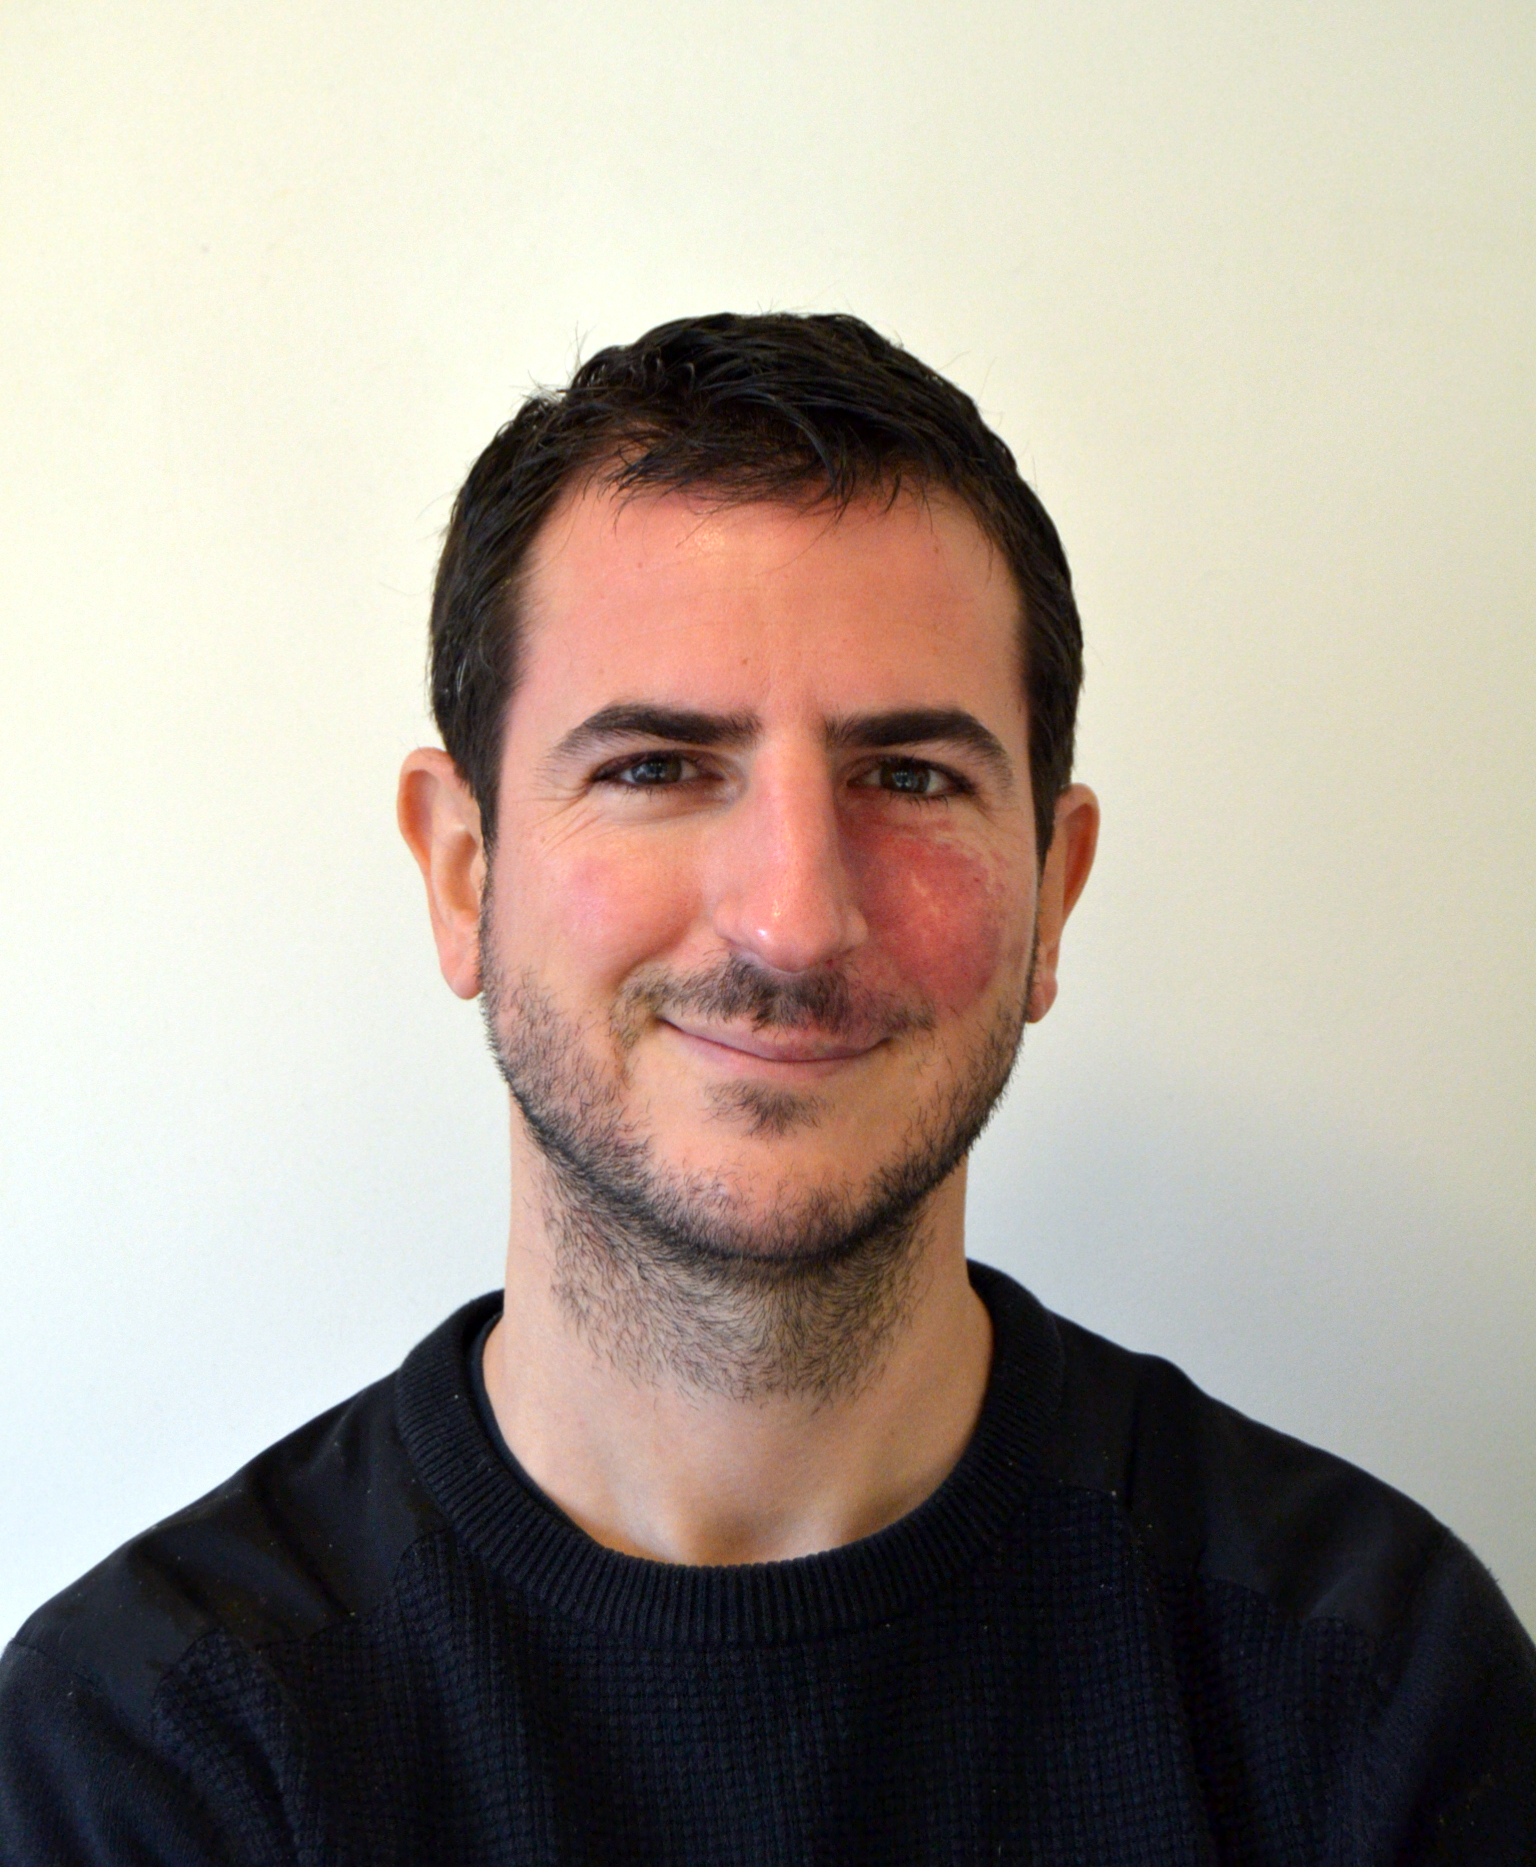
\includegraphics[width=5cm]{Javi_foto_curriculum_gimp_crop}};
\end{tikzpicture}

\section{Personal Information}
\cvline{Date of birth}{March 26, 1986}
%\cvline{Place of birth}{Salamanca, Spain}
%\cvline{Sex}{Male}
\cvline{Nationality}{Spanish, German}
\cvline{Email}{jmontejo@cern.ch}

\vspace*{5mm}




\section{Education and Research Positions}
\cventry{2017 - today}{CERN Staff Physicist}{}{}{
\newline{}L1Calo algorithm and performance coordinator.
\newline{}SUSY R-parity violating and long-lived subgroup convener.
\newline{}Trigger menu coordinator.
\newline{}Trigger coordination scientific secretary.}{}
\cventry{2015 - 2017}{CERN Fellow}{}{}{\newline{}SUSY third-generation subgroup convener.}{}
\cventry{2012 - 2015}{Ph.D.,}{Universitat Aut\'onoma de Barcelona,}{Spain.}{\newline{}
ATLAS thesis award, Springer thesis award.}{}
\cventry{2011 - 2012}{M.Sc. in High-Energy Physics,}{Universitat Aut\'onoma de Barcelona,}{Spain.}{}{}
\cventry{2005 - 2011}{B.Sc. in Computer Science,}{Universidad de Salamanca,}{Spain.}{\newline{}
Extraordinary Graduation Award.}{}
\cventry{2005 - 2010}{B.Sc. in Physics,}{Universidad de Salamanca,}{Spain.}{\newline{}Extraordinary Graduation Award.\newline{}National Award for Excellence in Academic Performance.}{}{}

\section{Trigger Experience}
\cvitem{}{I have contributed to the ATLAS trigger menu group throughout Run~2, initially as trigger menu expert and menu on-call, and during 2018--2019 as trigger menu coordinator. As such I was in charge of the menu during the intense period of special runs in 2018, including low-$\mu$, high-$\beta^*$, AFP runs and the Heavy-Ion run. After the data-taking period I defined the first baseline menu for Run~3, presented at the 2019 Trigger Workshop. Besides the menu composition, I contributed to dedicated studies in order to ensure that the trigger menu being designed would respect all the hardware and cabling constraints.
}
\cvitem{}{As part of my effort to improve the Run~3 triggers, I am currently L1Calo algorithm and trigger performance coordinator. My goal is to maximize the performance and rate gains from the phase-I L1Calo system, exploiting the capabilities of the new system to its full potential.
}

\section{Research Experience}

\cvitem{{Run~2: SUSY}}{
The large increase in energy and luminosity at the start of Run~2 made it the perfect moment to embark on BSM searches, where my main interest lies in natural SUSY models, both in R-parity conserving (RPC) and in violating (RPV) scenarios.
\begin{itemize}
%\item Searches for top squarks in final states with one isolated lepton, with \href{http://journals.aps.org/prd/abstract/10.1103/PhysRevD.94.052009}{3.2 fb$^{-1}$},  \href{https://atlas.web.cern.ch/Atlas/GROUPS/PHYSICS/CONFNOTES/ATLAS-CONF-2016-050}{14 fb$^{-1}$}, and  \href{https://link.springer.com/article/10.1007/JHEP06(2018)1089}{36 fb$^{-1}$}
%\item \href{https://link.springer.com/article/10.1007\%2FJHEP09\%282017\%29088}{Search for new phenomena in a lepton plus high jet multiplicity final state}, and its \href{https://link.springer.com/article/10.1007/JHEP05(2019)142}{reinterpretation in four-top final states from mediator-based dark matter models}.
%\item \href{https://atlas.web.cern.ch/Atlas/GROUPS/PHYSICS/CONFNOTES/ATLAS-CONF-2018-003/}{Reinterpretation of searches for supersymmetry in models with variable R-parity-violating coupling strength}. 
\item Searches for top squarks in final states with one isolated lepton, with 3.2 fb$^{-1}$[\coloredLink{http://journals.aps.org/prd/abstract/10.1103/PhysRevD.94.052009}{1}], 14 fb$^{-1}$[\coloredLink{https://atlas.web.cern.ch/Atlas/GROUPS/PHYSICS/CONFNOTES/ATLAS-CONF-2016-050}{2}] and 36 fb$^{-1}$[\coloredLink{https://link.springer.com/article/10.1007/JHEP06(2018)108}{3}].
\item Search for new phenomena in a lepton plus high-jet-multiplicity final state [\coloredLink{https://link.springer.com/article/10.1007\%2FJHEP09\%282017\%29088}{4}], and its reinterpretation in four-top final states from dark-matter models [\coloredLink{https://link.springer.com/article/10.1007/JHEP05(2019)142}{5}].
\item Reinterpretation of searches for supersymmetry in models with variable R-parity-violating coupling strength [\coloredLink{https://atlas.web.cern.ch/Atlas/GROUPS/PHYSICS/CONFNOTES/ATLAS-CONF-2018-003/}{6}].
\end{itemize}
}

%\cvitem{\textbf{Run~1: $\bm{\ttH(\bbbar)}$ and BSM $\bm{\ttbar\bbbar}$}}{
\cvitem{{Run~1: ttH(bb) and BSM ttbb}}{
The main topic of my Ph.D. work was searches in the \ttbar\bbbar\ final state, both in the SM (\ttH) and BSM with vector-like top partners, and scalar top partners.
\begin{itemize}
\item Search for the Standard Model Higgs boson produced in association with top quarks and decaying into \bbbar\ [\coloredLink{http://dx.doi.org/10.1140/epjc/s10052-015-3543-1}{7}].
\item  Search for production of vector-like quark pairs and of four top quarks  [\coloredLink{http://dx.doi.org/10.1007/JHEP08(2015)105}{8}].
\item ATLAS Run~1 searches for direct pair production of third-generation squarks [\coloredLink{http://dx.doi.org/10.1140/epjc/s10052-015-3726-9}{9}].
\end{itemize}
}

\section{Personal Statement}
\cvitem{}{
After the very successful Run~2 period, the trigger system is buzzing with developments, with the readiness for Run~3 as its main focus. The phase-I upgrades of L1Calo, L1Topo, L1Muon, NSW and MUCTPI will provide the trigger with new tools to face the challenging LHC environment, but even more important, new capabilities to boost the physics output. The ongoing work on the upgraded systems should ensure a fast and thorough commissioning of the trigger after the restart of data-taking in 2022. 
}
\cvitem{}{The priority for the trigger should be to maximize the physics potential of ATLAS. To do so, it will have to provide efficient data-taking for physics from day one, while the commissioning work prepares the path for a smooth and transparent transition to the upgraded systems before LHC reaches its peak luminosity. 
%three fronts, physics data-taking from day 1, guarantee stability for combination with Run~2, open new phase-space
%}
%\cvitem{}{
As we already experienced during Run~2, an apparently stable trigger is only achieved through a constant cycle of improvements and adaptation to changing LHC conditions and innovative offline techniques. The trigger must keep up with the evolving scenarios and eventualities that might arise, in order to guarantee a consistent dataset to be combined with that of Run~2. At the same time, it should maximize the gains from phase-I upgrades, which will allow us to accommodate new triggers targeting unexplored phase-space. 
}
\cvitem{}{If elected I would build on the organisation model used for the Trigger Activity since the start of Run 2, that has worked very well. I'd like to address also the challenges of attracting and retaining gifted young colleagues to work in the Trigger Activity, and making sure that their essential contributions are recognised in the Collaboration and beyond. 
}
\cvitem{}{
I would be thrilled and honoured to take up the challenges of (Deputy) Trigger Coordinator during the demanding and exciting years ahead of us, aiming to continue the successful operation of the ATLAS trigger while preparing for HL-LHC.
}

\end{document}


%% end of file `template.tex'.
